\chapter{Methodology}
\label{chap:metho}

Bridging the gap between unstructured design intent and formal model conditioning, Imagin3D operates as an orchestration system that translates moodboard layouts into precise signals for 3D generative models. This chapter first details the methodological rationale underpinning the system's design. Subsequently, it examines the frontend interface, specifically, the element modalities, spatial positioning, and clustering mechanisms that enable users to construct moodboards. Finally, the chapter outlines the core functionality of Imagin3D, distinguishing between the generation and adaptation workflows before detailing the overarching architecture and processing pipeline.

\section{Methodological Rationale}

Prior to detailing the interface and operational flow, it is necessary to contextualize the architectural decisions driving this framework. As discussed in the related work, various approaches exist for integrating external control signals into generative models; thus, justifying the selected methodology is a critical foundational step.

The transition from 2D-supervised to natively 3D-conditioned generation significantly improved output quality, but it consequently invalidated the use of 2D-based ControlNets on 2D primitives. While developing 3D-native ControlNets, such as those utilized in Hunyuan3D-Omni, remains possible, this approach strictly requires dimensionality matching between the conditioning signal and the output (e.g., mapping 3D bounding boxes to 3D geometry). Furthermore, training these networks relies on massive, paired datasets. Traditional control signals, such as bounding boxes, voxel grids, or skeletal rigs, can be programmatically extracted from existing 3D models to automatically generate these paired training sets. Therefore, the viability of ControlNet-style architectures depends on two strict prerequisites: automated data extraction and dimensional parity between inputs and outputs.

Moodboard-driven 3D generation lacks both of these prerequisites. The creation of a moodboard from a finished 3D object cannot be reliably automated, and the unstructured, abstract nature of a moodboard does not natively translate into a spatial 3D signal. Consequently, direct ControlNet implementations are unfeasible for this task. An alternative approach involves integrating lightweight adapters into the 3D generation models; however, this faces the exact same insurmountable data scarcity problem, as reverse-engineering a paired dataset mapping a text prompt and a moodboard to a final 3D asset cannot be automated.

To circumvent the issue of data scarcity, one might theoretically curate a small-scale paired dataset to train a custom adapter. However, such an approach is practically unviable. Constrained by the limited size and diversity inherent to manual data curation, this type of adapter would inevitably suffer from severe overfitting. Consequently, it would exhibit poor generalization capabilities, consistently failing to interpret novel concepts, niche styles, or complex visual metaphors that fall outside its restricted training distribution. Furthermore, the manual labor required to construct this dataset and engineer a bespoke training pipeline would represent a prohibitively inefficient expenditure of resources. Ultimately, this effort would merely provide empirical validation for an established theoretical constraint: imposing an adapter-based architecture onto unstructured moodboard data is fundamentally incompatible.

To resolve this, this research adopts an intelligent orchestration paradigm. This method translates diverse input modalities into a unified textual space, enabling the system to evaluate them holistically while preserving the semantic weight conveyed through their scale and spatial clustering. This conversion occurs in the text domain rather than through latent embeddings to avoid the generalization limitations inherent to multimodal spaces. As previously noted, while unified embedding spaces successfully align broad text, image, and 3D geometry categories, they become brittle when processing unseen data, niche styles, or abstract visual metaphors, leading to unpredictable relevance filtering.

Operating in this textual space allows the system to weigh the relative importance of moodboard elements by comparing them directly against the user's textual prompt. From these weighted elements, a comprehensive global prompt is synthesized. This prompt, alongside the original visual reference materials, is processed by a 2D generative model to produce an intermediate output, which is subsequently fed into the final 3D generative pipeline.

Ultimately, this orchestration leverages the zero-shot reasoning capabilities of existing large models to convert unstructured moodboards into the specific conditioning signals natively supported by current 3D generators. While this staged pipeline inherently increases inference time compared to trained end-to-end solutions like lightweight adapters or dedicated ControlNets, it significantly enhances user editability between steps and successfully preserves the nuanced design intent embedded within the original moodboard.

\section{The Moodboard Interface}

Fundamentally, a moodboard is a curated visual composition—a collage integrating images, text, and object samples to communicate a cohesive design intent.

\begin{figure}[H]
\centering
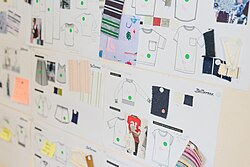
\includegraphics[width=0.5\textwidth]{images/moodboard-example.jpg}
    \caption[Moodboard example]{An example of a physical moodboard}
\end{figure}

Within the context of this research, we adapt this concept into an interactive digital moodboard situated on a 2D canvas. Users can populate this workspace with diverse input modalities, explicitly defining their spatial positioning and scale to convey relative importance. Furthermore, the interface supports explicit clustering, allowing users to spatially group multiple elements to signify a shared theme or conceptual relationship. The following subsections will detail the specific input modalities supported by the system, as well as the semantic weight carried by spatial layout, scaling, and clustering.

\subsection{Input Modalities}

Rather than relying on a solitary text or image prompt, a moodboard framework captures a substantially broader spectrum of design intent. It achieves this by integrating multiple input modalities, each capable of conveying information in distinct and highly specific ways. Visual conceptualization can be achieved through a wide variety of expressive modalities. The specific selection for our frontend interface reflects a deliberate balance between practical utility and technical feasibility. It aligns with standard 3D design workflows and omits irrelevant media such as audio, while accounting for the strict technical constraints governing which signals can be effectively processed and encoded to steer the underlying 3D generative model.

\paragraph{3D Models} Existing 3D models can be placed on the moodboard as reference geometry. They provide explicit structural guidance, allowing the system to capture proportions, spatial relationships, and shape priors that would be difficult to communicate through other modalities. These references can serve multiple purposes: as full object templates that should be closely reproduced, as partial elements that guide specific aspects of the generation, or as geometric constraints that bound the solution space. For instance, a user might include a reference chair model to establish desired proportions while leaving material and stylistic details to be determined by other moodboard elements.

\paragraph{Video} Video input allows users to communicate motion, atmosphere, temporal evolution, or sequences of perspectives that reveal object structure. Dynamic content offers unique advantages for 3D generation, as it inherently captures multi-view information and can convey qualities like lighting changes or animated textures. However, processing full video sequences would be computationally prohibitive and introduce redundancy. To address this, the system performs intelligent frame sampling based on visual change detection. Frame-to-frame differences are computed using perceptual metrics and select keyframes that represent meaningful visual transitions. These keyframes are then treated as individual image inputs, preserving the essential information while maintaining efficiency.

\paragraph{Images} Still images serve as the primary visual references for style, texture, lighting, and composition. They form the backbone of most moodboards and bridge other modalities by providing concrete visual examples that complement abstract specifications. Images can communicate complex aesthetic qualities, such as material properties, lighting conditions, or stylistic treatments, that would require extensive text descriptions to approximate. Their versatility makes them suitable for representing everything from photographic references to artistic inspirations to technical diagrams.

\paragraph{Text} Text input provides semantic and descriptive information that cannot easily be captured visually. This includes design intent, material descriptions, functional requirements, conceptual notes, and contextual information about intended use or target audience. Text serves a complementary role to visual inputs: where images show "how something should look," text can specify "what something should be" or "why certain choices matter". Short labels can annotate specific elements, while longer descriptions can provide overarching guidance for the entire generation.

\paragraph{Color Palettes} Color palettes summarize mood, atmosphere, and tonal relationships in a compact, interpretable form. They can be inserted manually by users selecting specific colors, or extracted automatically from images. Palettes serve multiple functions: they provide direct guidance about desired color schemes, help establish emotional tone, and enable the system to identify thematic consistency across disparate visual references. Color information also facilitates coherent material assignment in generated 3D models, ensuring that the final output respects the intended chromatic harmony.

\subsection{Spatial Composition and Clustering}

In a digital moodboard, spatial layout acts as an explicit form of visual programming. Rather than relying on complex mathematical distance heuristics, the system extracts two highly deliberate user actions to dictate how disparate influences are weighted and blended: element scale and explicit clustering. 

First, the relative bounding box size of an element acts as its implicit weight. Larger items visually dominate the hierarchy and receive higher priority during prompt synthesis. This allows users to intuitively emphasize primary structural templates by scaling them up, while shrinking secondary textural details to minimize their structural influence on the final geometry. 

Second, users can manually group related elements to form cohesive clusters. This explicit clustering enables hierarchical composition, allowing the orchestration pipeline to process the cluster as a single, consolidated thematic concept rather than a collection of disparate inputs. Ultimately, this structured grouping significantly enhances the interpretability and accuracy of the system.

\section{The Imagin3D Architecture}

The underlying orchestration required to guide generative models using a spatial moodboard involves a multi-stage pipeline. This section details the complete architectural flow, from unstructured canvas inputs to the final realized 3D asset.

\subsection{Modes of Operation: Generation and Adaptation}

Imagin3D supports two primary operational flows to accommodate different stages of the creative process: from scratch generation and reference-based adaptation. While both workflows share the same foundational architecture and rely heavily on the moodboard for stylistic and structural cues, they differ fundamentally in their initial state. 

Generation represents a "cold start" scenario. It builds a 3D asset entirely from scratch, relying exclusively on the user's text prompt and the curated visual influences present on the moodboard. Adaptation represents a "hot start" approach. Instead of a blank slate, it builds upon a foundational reference subject, taking in both a specific base target (such as a core text description, a 2D image, or an existing 3D model) and a modifying text prompt. 

Architecturally, this distinction primarily dictates how instructions are formulated for the underlying large language and vision models throughout the pipeline. While a generation flow simply prompts the models to synthesize a concept based on the overarching text, an adaptation flow fundamentally restructures these internal prompts, explicitly instructing the models to evaluate the provided baseline subject and modify its style, geometry, or material properties to align with the adaptation prompt and moodboard context. 

This dual methodology provides users with two distinct degrees of control: they can either explore entirely novel forms emergent from their collective references, or they can tightly constrain the generation by anchoring it to a specific pre-existing object and using the moodboard purely as a stylistic guide.

\subsection{The Pipeline Orchestration}

\begin{figure}[H]
\centering
    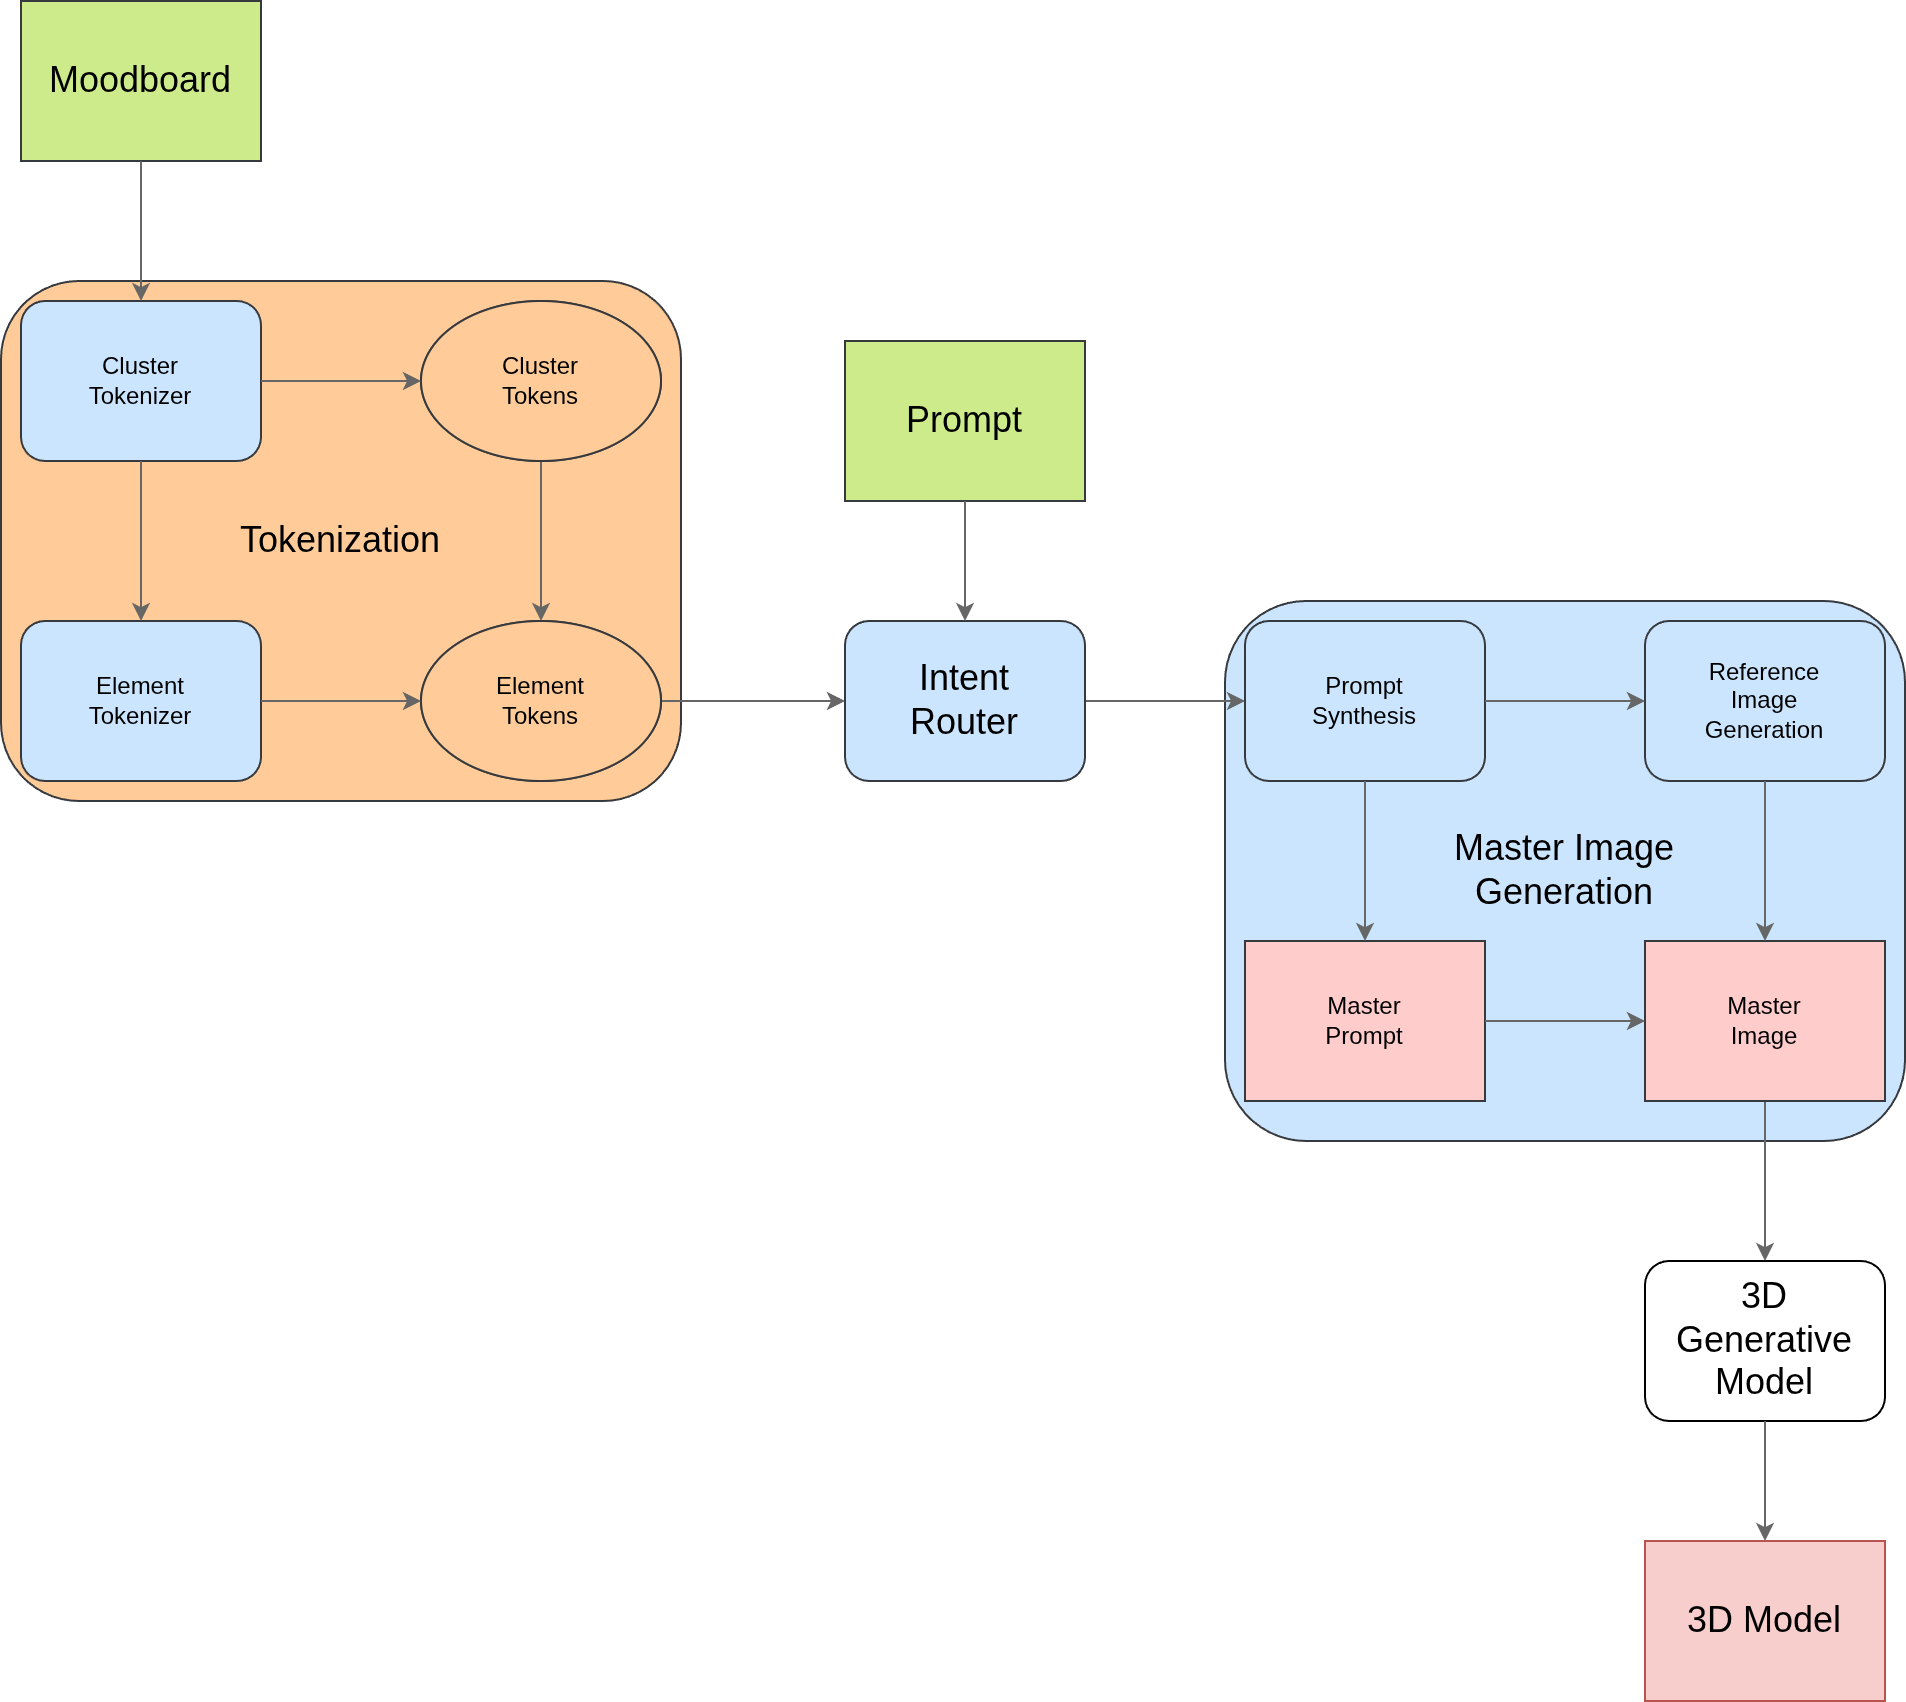
\includegraphics[width=\textwidth]{images/new_architecture.png}
    \caption{The general architecture of Imagin3D}
\end{figure}

Before delving into the specific technical mechanisms of each step, it is helpful to view the pipeline from a high level. The general process begins by ingesting the diverse content of the moodboard and standardizing it. Next, a tokenization phase converts these elements into structured semantic descriptors, explicitly capturing organizational queues like clustering and spatial scale. Following this, the system filters out irrelevant noise by weighting each element against the explicit prompt provided by the user. The highest-scoring references, alongside their linguistic tokens, are then fused to synthesize a unified master prompt and a subsequent master image. This 2D intermediate representation serves as the definitive visual control signal required to guide the 3D generation into the correct structural direction.

To contextualize the technical pipeline detailed in the following sections, it is necessary to establish the foundational inputs guiding the system. Figure \ref{fig:moodboard_input} displays a populated moodboard interface, containing the initial visual references, spatial scales, and conceptual clusters established by the designer. Concurrently, Figure \ref{fig:prompt_input} presents the explicit generation prompt orchestrating the active creative task. Together, these two foundational conditions provide the continuous source material driving every subsequent algorithmic transformation and will serve as the origin point for all intermediate outputs showcased throughout the remainder of this section.

\begin{figure}[H]
\centering
    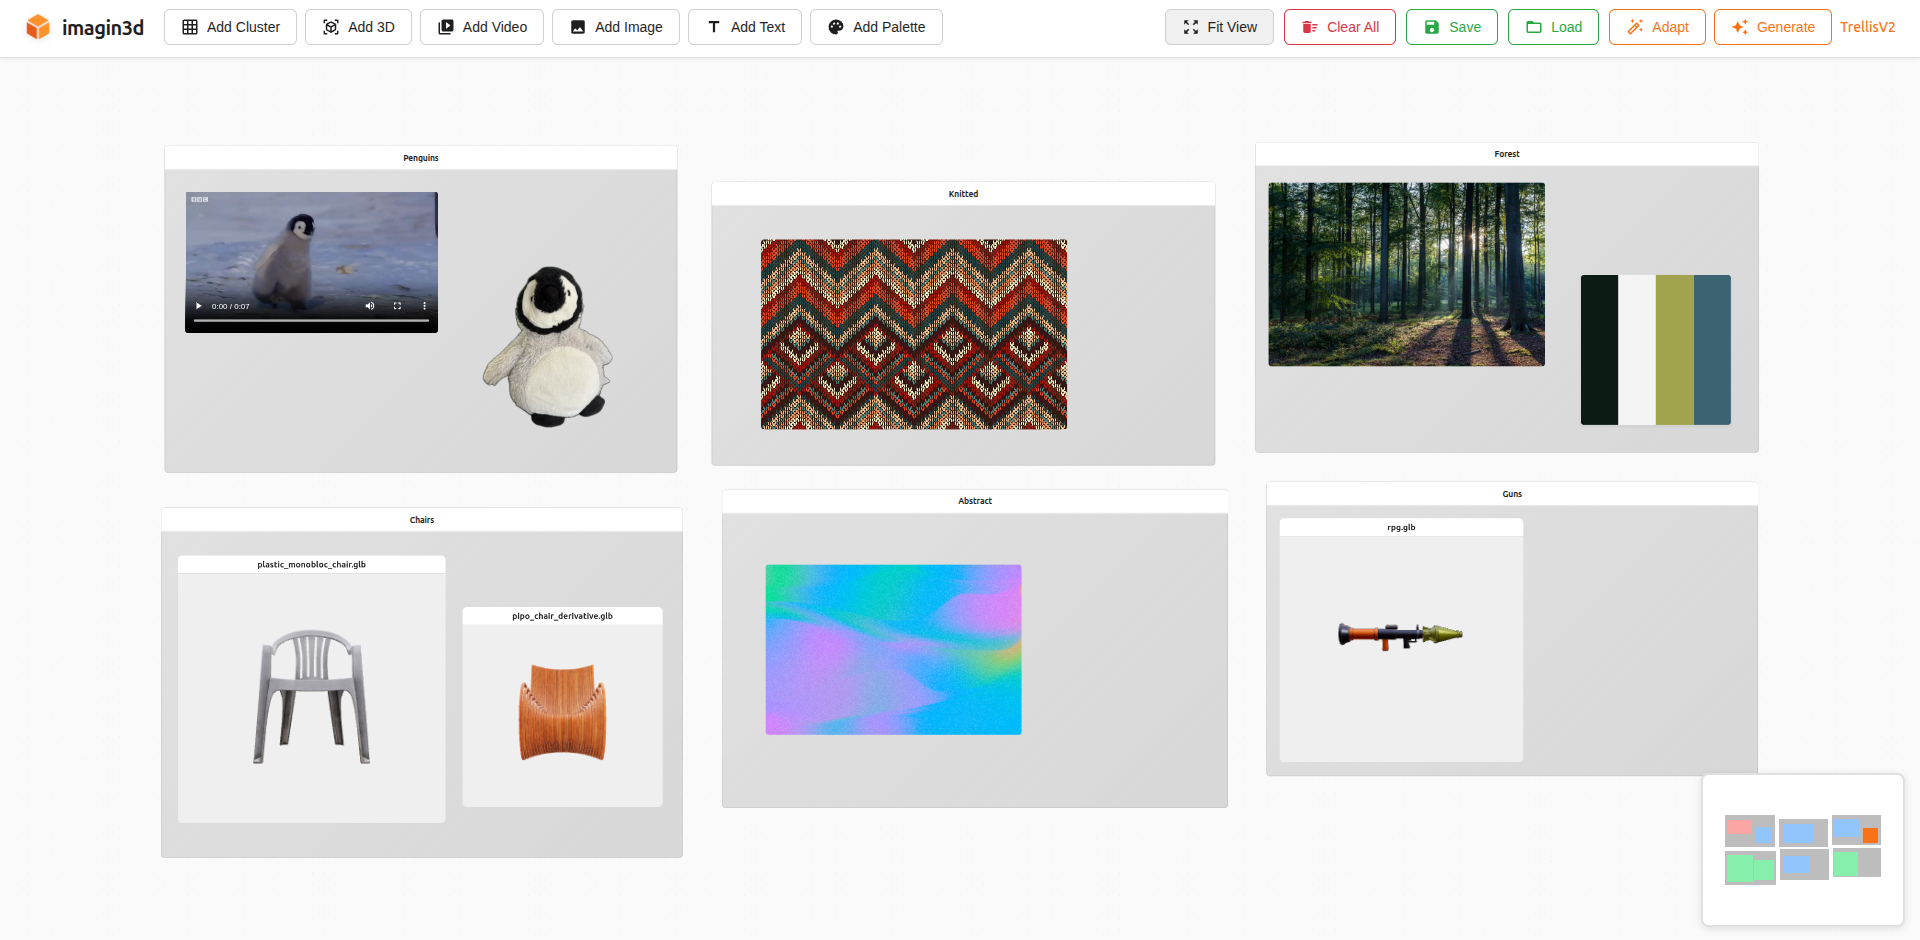
\includegraphics[width=\textwidth]{images/multimodal-ingestion.png}
    \caption{A screenshot of a populated moodboard in the Imagin3D interface establishing the visual input context.}
    \label{fig:moodboard_input}
\end{figure}

\begin{figure}[H]
\centering
    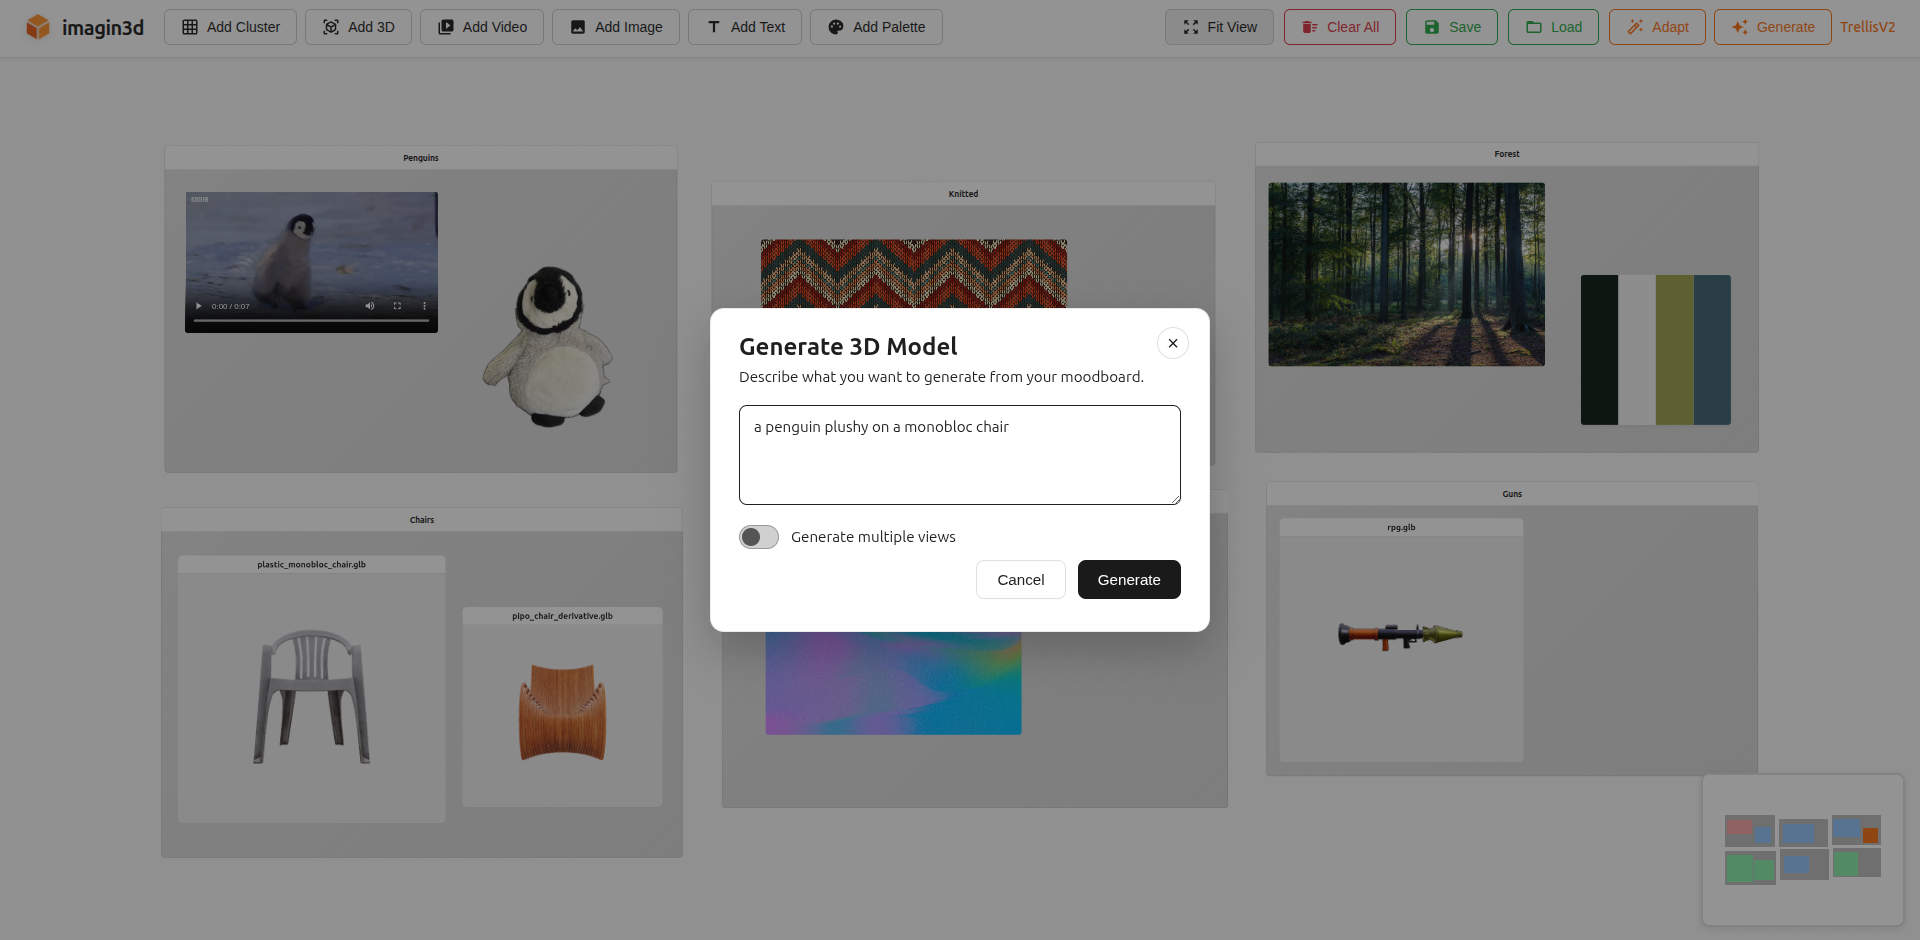
\includegraphics[width=\textwidth]{images/prompt.png}
    \caption{A screenshot of the corresponding generation prompt driving the active orchestration pipeline.}
    \label{fig:prompt_input}
\end{figure}

\subsubsection{Multimodal Ingestion}

The first active step in the pipeline is the ingestion of diverse multimodal content from the moodboard. Because human designers naturally coordinate their ideas using a variety of formats, the system must standardize these inputs into a digestible format. Text elements and color palettes can be extracted directly as semantic strings, but spatial and temporal elements require aggressive normalization. For instance, if a user places an existing 3D model onto the board, the backend engine automatically renders it from multiple angles to create representative 2D views. Similarly, uploaded videos are processed to extract discrete, highly representative keyframes. By projecting complex spatial and temporal elements into static 2D imagery, the system establishes a unified visual language that vision-language models can reliably and consistently interpret in subsequent analytical stages.

\subsubsection{Semantic Extraction and Tokenization}

Following the ingestion and visual normalization of all elements, the system executes a critical tokenization phase where the various inputs are translated into rich semantic descriptors. To preserve the hierarchical relationships established on the moodboard, this data extraction follows a precise sequential methodology.

First, the system scans the entire moodboard to identify any elements that the user has explicitly grouped into spatial clusters. For every cluster detected, a dedicated clusterer agent evaluates the collective assembly to generate a unified thematic descriptor. This initial sweep ensures that every grouping on the canvas is assigned a localized, overarching context before individual elements are processed. 

Subsequently, a specialized descriptor agent systematically analyzes each individual moodboard element to generate its highly structured semantic descriptor, formally defined as a design token. During this element-level analysis, the system explicitly incorporates both the previously established cluster context (if the element belongs to one) and the element's spatial scale on the canvas. By integrating the surrounding thematic context with the intuitive weight of the user-defined scale, the resulting semantic descriptors capture a deeply nuanced visual representation of the asset relative to its environment. This structured sequence ensures that subjective, multimodal inputs are reliably translated into an explicit semantic format, allowing the system to mathematically process creative intent without sacrificing contextual nuance.

Computationally, a design token operates as a multifaceted data structure necessitated by a fundamental architectural challenge: AI agents cannot intrinsically interpret a boundless spatial canvas, nor can they directly compare fundamentally different raw media formats (such as evaluating a 3D mesh against a text passage) on equal footing. To resolve this bottleneck, the design token architecture acts as a universal currency that homogenizes disparate modalities into a predictable format. It achieves this by independently addressing the three core requirements of spatial reasoning and multimodal design, encompassing the following exact components:

\begin{itemize}
    \item \textbf{Semantic Payload:} To allow different media types to be compared, the system must extract their meaning into a shared format. The token achieves this by storing a concise title and a comprehensive description. The processing engine dynamically adapts to the input modality to generate this payload: standard large language models efficiently process pure text constraints and color palettes, whereas vision-language models analyze structurally complex inputs such as images, video keyframes, and rendered three-dimensional geometry. 
    \item \textbf{Spatial Characteristics:} Because the semantic payload strips away the visual interface, the token must inherently preserve the spatial framework of the original moodboard. It does so by explicitly recording the precise coordinates and multidimensional scale of the element on the canvas. This allows downstream components to independently prioritize an element based purely on the physical size the user assigned it, before even reading the text description.
    \item \textbf{Algorithmic Anchors:} Finally, to mathematically process these inputs through generative pipelines, the tokens are explicitly designed to act as compute anchors, storing continuous vector embeddings and relevance weights explicitly assigned during the routing phase.
\end{itemize}

This robust architecture ensures that upon tokenization, the system accurately bridges the visual, spatial, and semantic domains. Without forcing the multimodal data into this highly explicit layout, intelligently orchestrating a multi-agent generative pipeline conditioned on a chaotic design board would be functionally intractable.

\subsubsection{Intent-Based Routing}

Before the moodboard content can be strictly fed into the generative framework, the system must determine which elements are actually relevant to the immediate task. A single moodboard may contain references spanning multiple distinct themes, styles, or concepts accumulated across an extended session. How relevance is determined depends on the active operational mode. During a pure generation flow, elements are scored on how well they align with the user's overarching text prompt. Conversely, during an adaptation flow, the intent router must evaluate the elements against both the adaptation prompt and the specific baseline subject being modified, determining whether a moodboard element provides relevant stylistic or geometric guidance for that particular transformation.

The intent routing system solves this by operating at multiple levels of granularity. First, at the cluster level, the system assesses whether entire thematic groups are relevant to the active task. Subsequently, at the element level, an intent router agent evaluates individual elements to generate a single, comprehensive relevance score. This unified calculation simultaneously accounts for the element's specific semantic alignment, its parent cluster's overall relevance, and its spatial characteristics from the design token, structurally prioritizing elements that are visually scaled up or clustered closely together. This singular score is then systematically populated as the initial algorithmic weight value directly within each element's respective design token. Crucially, before the pipeline advances, these calculated weights are exposed within the user interface, allowing the designer to manually fine-tune or override the agent's assessment to ensure perfect alignment with their specific creative intent.

\begin{figure}[H]
\centering
    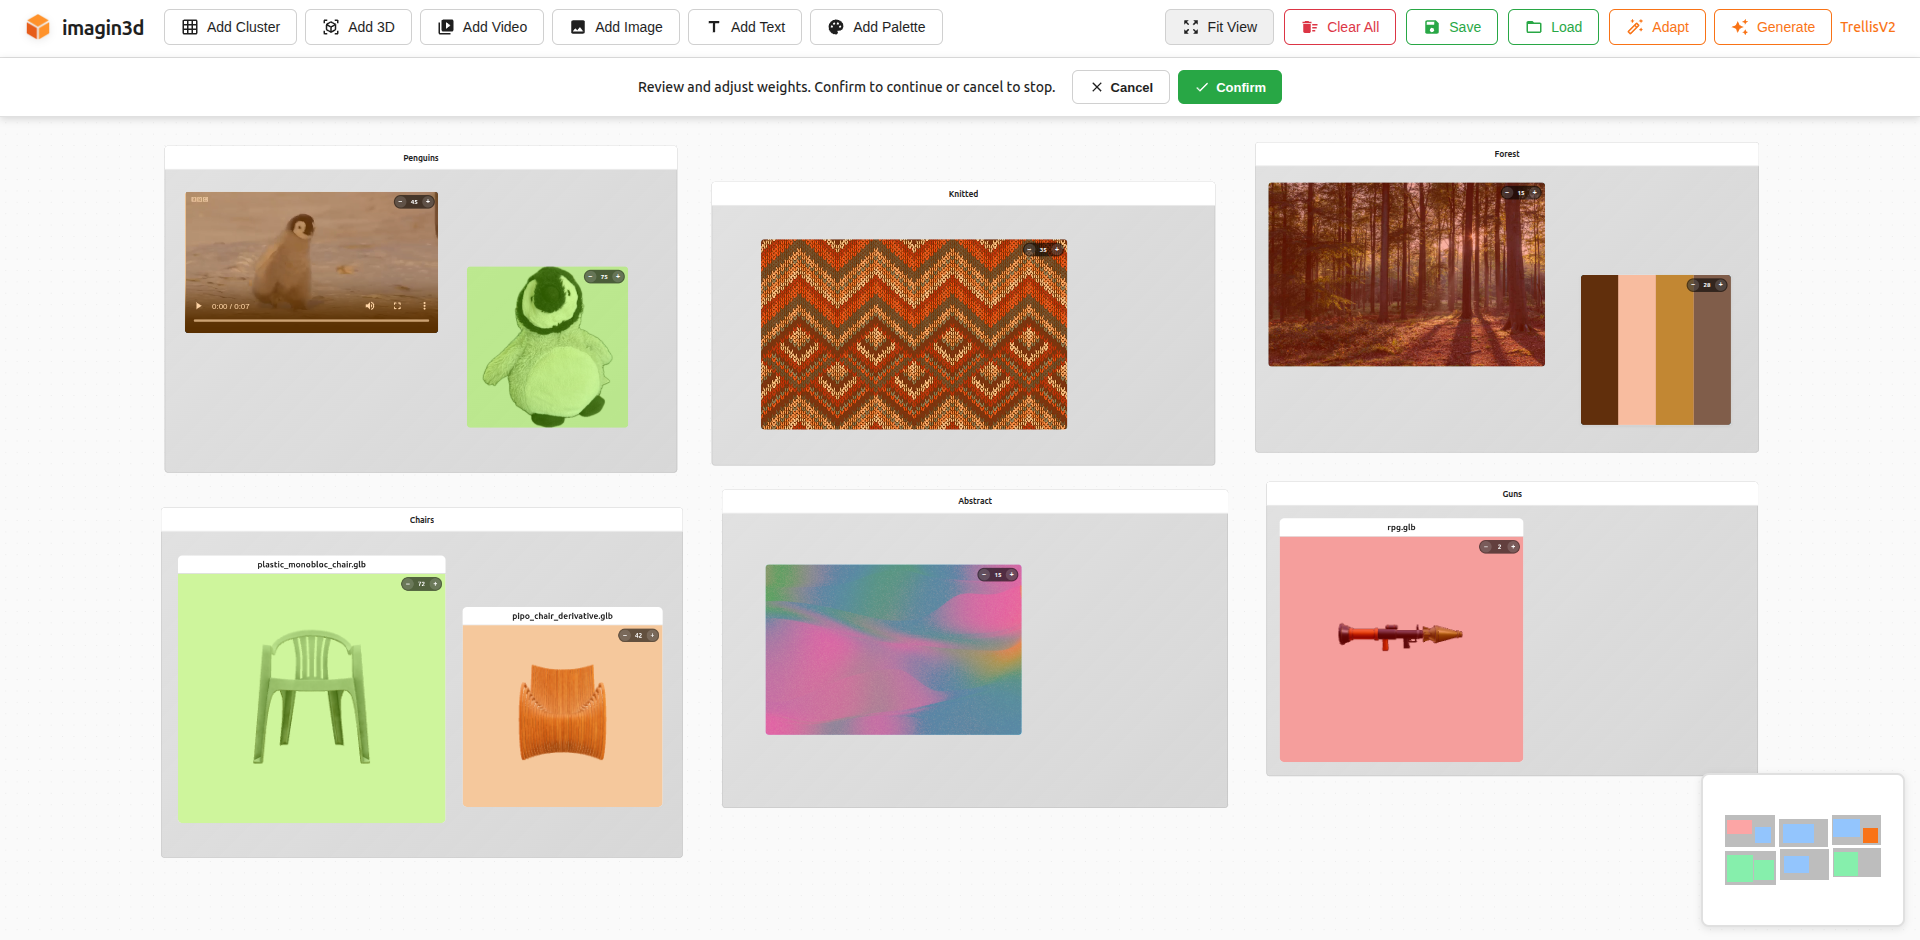
\includegraphics[width=\textwidth]{images/intent-routing.png}
    \caption{A screenshot of the moodboard interface visually demonstrating the routing process.}
\end{figure}

The output of this active routing process is a weighted representation of the moodboard where each element and cluster carries a definitive relevance score. To prevent conflicting or dilute influences from muddying the final output, the system applies a strict relevance threshold, filtering out any elements scoring below fifty percent. The remaining highly relevant moodboard items become the focused input fed to the synthesis pipeline.

\subsubsection{Master Visual Synthesis}

With the irrelevant elements stripped away, the system bridges the gap between fragmented inspiration and a cohesive concept through master visual synthesis. This is a two-part process involving prompt compilation and 2D image generation. First, a specialized prompt synthesizer agent gathers the high-scoring design tokens, their cluster descriptors, the user's original text prompt, and the associated visual style images. The agent cognitively fuses these filtered constraints into a single, comprehensive text prompt. This "master prompt" encapsulates the exact geometric structure requested by the user while gracefully weaving in the aesthetic nuances, color schemes, and image references extracted directly from the moodboard.

Immediately following this compilation, the synthesized master prompt is passed to a visualizer agent. This agent acts as an advanced text-to-image generator, consuming the master prompt alongside the collected style images to generate a dense 2D intermediate representation of the user's intended 3D object. In the case of an adaptation flow, the original base image is also supplied as strict structural scaffolding. This "master image" serves as a highly interpretable, verifiable bridge between the user's abstract conceptual moodboard and the physical 3D space, establishing an unambiguous visual target before expensive 3D processing begins. 

\begin{figure}[H]
\centering
    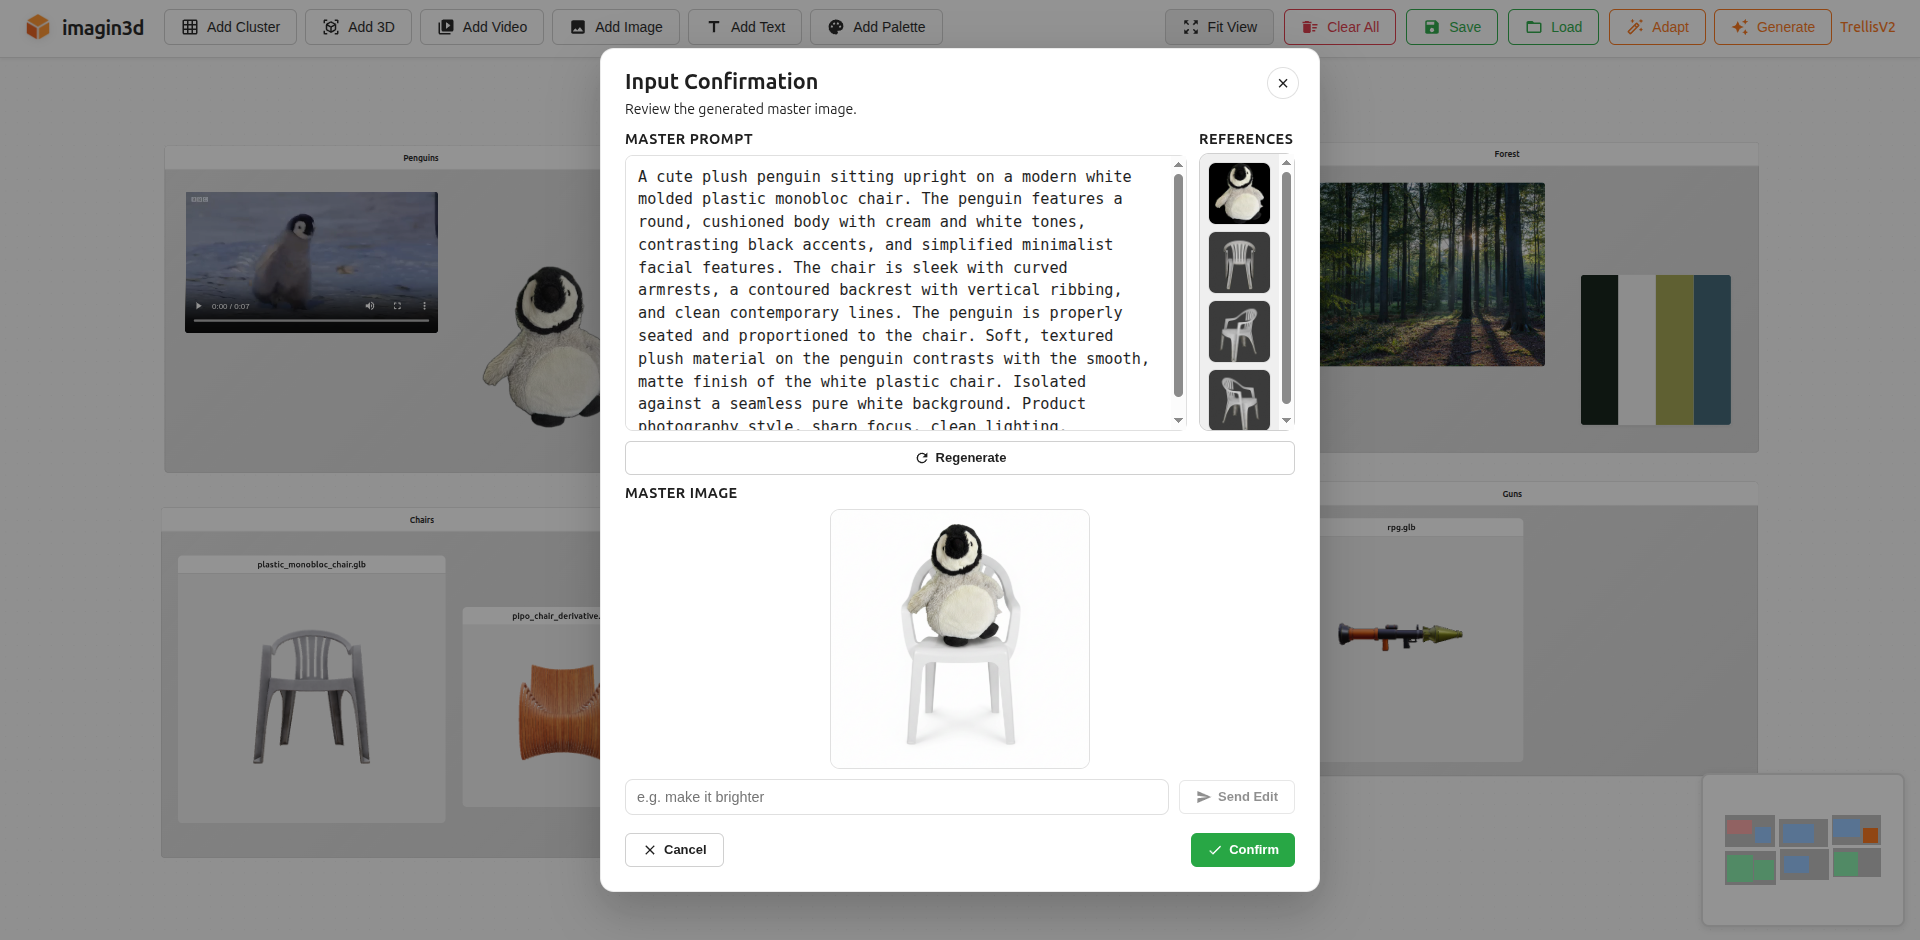
\includegraphics[width=\textwidth]{images/master-visual.png}
    \caption{A screenshot showcasing the generated master prompt text juxtaposed with the resulting master image.}
\end{figure}

Crucially, to maintain ultimate creative control, the underlying master prompt is exposed within the interface for manual editing, allowing the user to iteratively regenerate the two-dimensional image until the result meets their exact aesthetic and structural specifications. Furthermore, direct visual edits and adjustments can be applied to the master image itself, providing a final layer of localized, pixel-perfect control prior to three-dimensional instantiation.

\subsubsection{3D Object Instantiation}

\begin{figure}[H]
\centering
    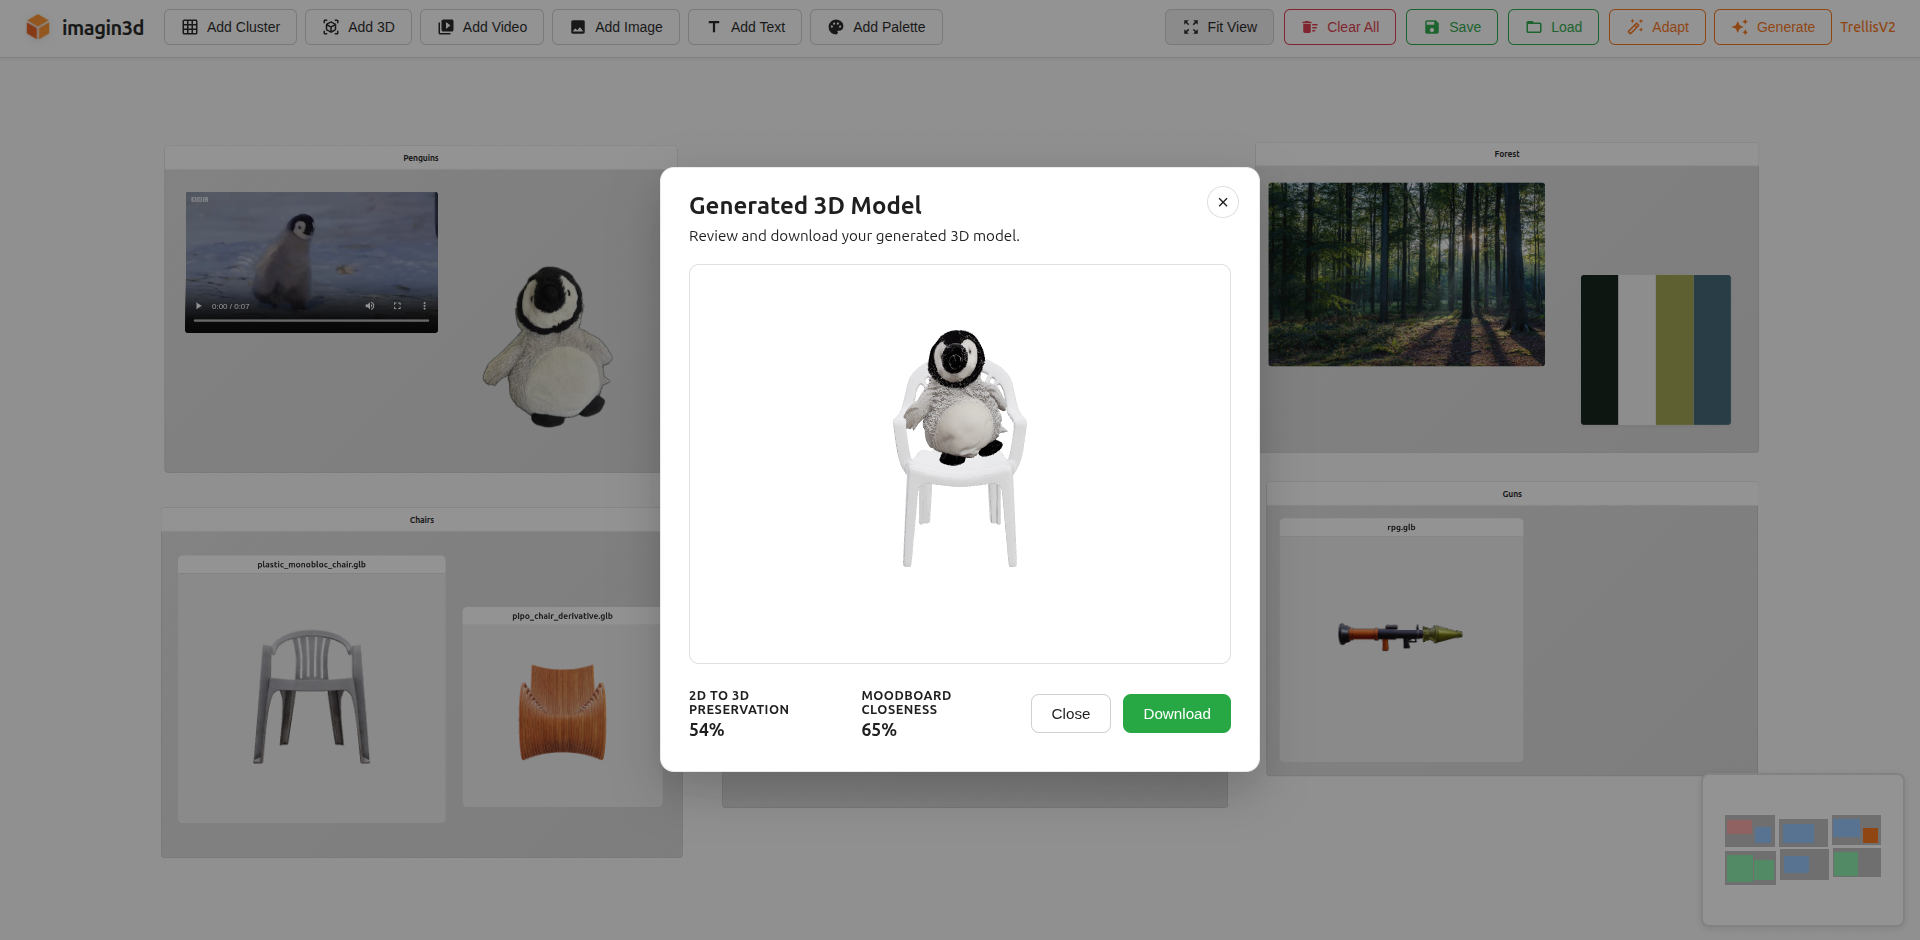
\includegraphics[width=\textwidth]{images/3D-object.png}
    \caption{A screenshot of the final 3D generated model.}
\end{figure}

In the final automated step, the master image serves as the explicit conditioning signal for the 3D generation engine. Using an advanced image-to-3D latent diffusion pipeline (such as the Trellis architecture), the system projects the 2D aesthetic of the master image into a fully realized 3D mesh. Because the master image has already done the heavy lifting of consolidating the user's disparate moodboard influences into one cohesive visual representation, the 3D model simply has to reconstruct the implicit geometry of that single image. The resulting generated mesh accurately reflects both the broad form requested in the prompt and the finely nuanced style curated on the original board.

\subsection{Tackling the Janus Problem with Multiview Mode}

While generating a single master image is computationally efficient and highly effective for many objects, it inherently lacks information about the occluded sides of the target geometry. This spatial ambiguity can occasionally force the 3D generative model to guess, leading it to hallucinate geometry or project conflicting frontal features onto the back of the model (frequently referred to as the Janus problem). 

\begin{figure}[H]
\centering
    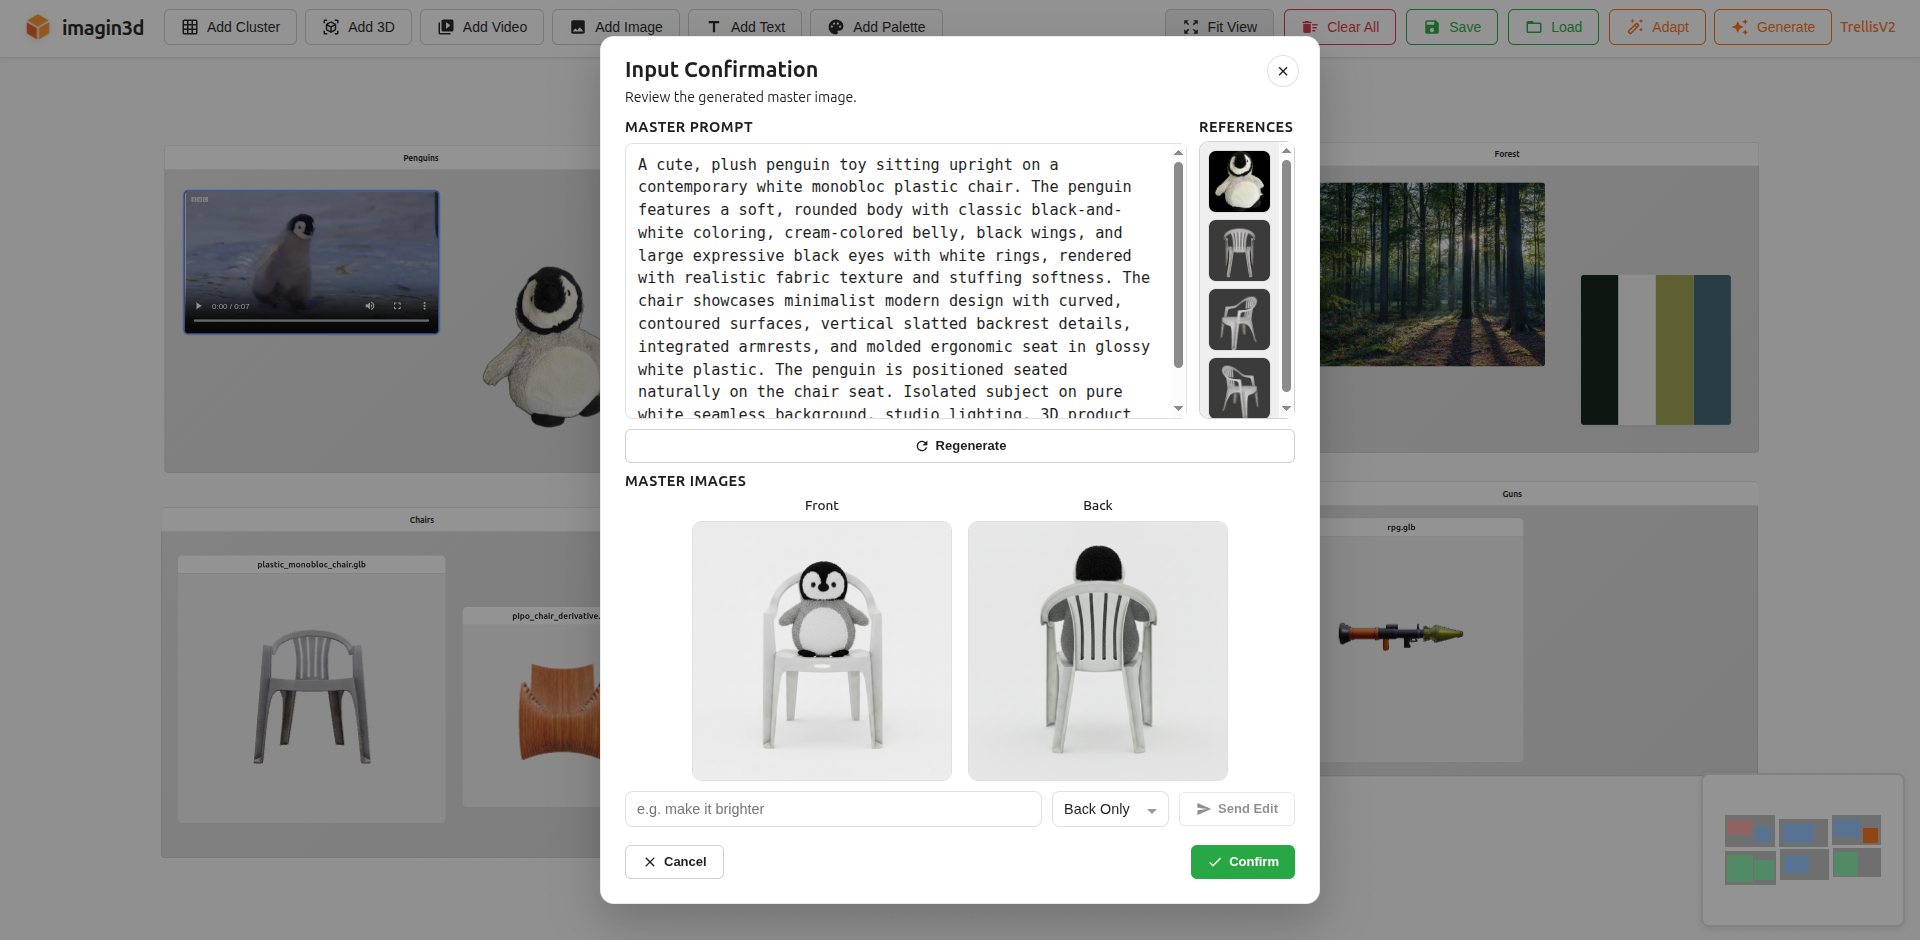
\includegraphics[width=\textwidth]{images/multiview.png}
    \caption{A alternative screenshot showcasing the generated master prompt text juxtaposed with the resulting multiview master image.}
\end{figure}

To mitigate this systematic limitation, Imagin3D introduces a dedicated Multiview Mode. In this advanced operational mode, the visualizer agent is explicitly instructed to generate two complementary master images illustrating both the front and the back views of the unified concept simultaneously. Crucially, both of these generated perspectives remain fully accessible for direct user editing. This total visibility ensures that the designer retains pixel-perfect control over every angle of the object, completely eliminating the issue of uneditable occluded regions. These multiple curated perspectives are then jointly fed into a multi-image conditioned 3D generation pipeline. By providing explicit visual supervision for the entire 360 degree object layout, this approach drastically improves geometric consistency and virtually eliminates common multi-view projection artifacts, resulting in a significantly more robust and structurally sound end product.